\documentclass{beamer}
\usetheme{Madrid}

%
% Choose how your presentation looks.
%
% For more themes, color themes and font themes, see:
% http://deic.uab.es/~iblanes/beamer_gallery/index_by_theme.html
%
\mode<presentation>
{
  \usetheme{Madrid}      % or try Darmstadt, Madrid, Warsaw, ...
  \usecolortheme{seahorse} % or try albatross, beaver, crane, ...
  \usefonttheme{default}  % or try serif, structurebold, ...
  \setbeamertemplate{navigation symbols}{}
  \setbeamertemplate{caption}[numbered]
} 

\usepackage[spanish]{babel}
\usepackage{amsfonts, amssymb, amsmath, amsthm, mathrsfs}
\usepackage[utf8]{inputenc}
\usepackage[T1]{fontenc}
\usepackage{ragged2e}
\usepackage{tikz}
\usetikzlibrary{calc,arrows.meta,positioning}

\usepackage{bbm}
\usepackage{derivative}
\newcommand{\abs}[1]{\left|#1\right|}
\newcommand{\norm}[1]{\left\lVert#1\right\rVert}
\newcommand{\ds}{\displaystyle}
\newcommand{\ind}{\mathbbm{1}}

\justifying

\usefonttheme{professionalfonts}

\makeatletter
\renewenvironment{proof}[1][\proofname]{%
  \par\pushQED{\qed}%
  \normalfont
  \topsep6\p@\@plus6\p@\relax
  \trivlist
  \item[\hskip\labelsep\itshape #1\@addpunct{.}]
}{%
  \popQED\endtrivlist\@endpefalse
}
\makeatother
\renewcommand{\qedsymbol}{$\blacksquare$}


\title[SVM]{Support Vector Machines (SVMs)}
\author{Fernando, Julia, Hugo y Mario}
\institute{UAM}
\date{24 de marzo de 2026}

\begin{document}

\begin{frame}
  \titlepage
\end{frame}

% Uncomment these lines for an automatically generated outline.
%\begin{frame}{Outline}
%  \tableofcontents
%\end{frame}

\section{Metodología}
\begin{frame}{Metodología}
    Nos hemos reunido presencialmente en tres ocasiones:
    \begin{enumerate}
        \item Estudiar la teoría vista en clase y la bibliografía principal (S. Shalev-Shwartz \& S. Ben-David (2014), \textit{Understanding Machine Learning: From Theory to Algorithms}) colectivamente.
        \item Plantear el trabajo y dividir en temas.
        \item Presentar al resto del grupo lo que se ha hecho por separado.
    \end{enumerate}

    \vspace{0.5cm}
    Uso de modelos del lenguaje para programar jupyter notebooks usando las librerías de \texttt{sklearn}. Cada uno ha usado el modelo y entorno que ha considerado.
\end{frame}


\section{SVMs}
\begin{frame}{Hard-SVM}
Consideramos un problema de clasificación binaria con clases $-1$ y $+1$.\\
\vspace{0.25cm}
Sea $D=\{(x_i, y_i)\}_{i=1}^m$ el conjunto de entrenamiento, donde $x_i \in \mathbb{R}^d$, $y_i \in \{-1, +1\}$.\\
\vspace{0.25cm}
\textbf{Objetivo:} Encontrar un hiperplano que separe las dos clases.\\
\vspace{0.25cm}
\begin{block}{Definición}
Decimos que $D$ es \textbf{separable por un hiperplano} si existe un hiperplano dado por $(w, b)$ tal que $y_i = sign(\langle w,x_i\rangle +b) \ \forall i \in \{1, \dots, m\}$, equivalentemente $y_i(\langle w,x_i\rangle +b) > 0 \ \forall i \in \{1, \dots, m\}$
\end{block}
\vspace{0.25cm}
\underline{Observación:} Si $D$ es separable por un hiperplano, hay infinitos hiperplanos separadores.\\
\vspace{0.25cm}
¿Cómo elegimos el hiperplano óptimo?
\end{frame}

\begin{frame}
\begin{block}{Definición}
Sea $D$ separable por un hiperplano. Definimos el \textbf{margen} de $D$ con respecto a un hiperplano $(w,b)$ (con \(\lVert w \rVert = 1\)) como $\gamma > 0$ tal que $y_i(\langle w, x_i \rangle +b) \ge \gamma \ \forall i \in \{1, \dots, m\}$ 
\end{block}
\vspace{0.5cm}
Tomamos el hiperplano separador con mayor margen,
$$\underset{(w,b) : \|w\|=1}{\text{arg máx}} \min_i |\langle w, x_i\rangle+b| \  \ \text{  sujeto a  } \ y_i(\langle w,x_i \rangle +b) > 0 \ \forall i$$
\begin{block}{Algoritmo Hard-SVM}
input: $(x_1,y_1), \dots, (x_m,y_m)$\\ \vspace{0.15cm}
solve: $(w_0,b_0) = \arg\min_{w, b}\|w\|^2$ sujeto a $y_i(\langle w,x_i\rangle+b)\geq 1$ $\forall i$\\ \vspace{0.15cm}
output: $w = \frac{w_0}{\|w_0\|}$, $b = \frac{b_0}{\|w_0\|}$
\end{block}
Se tiene que $\gamma = \frac{1}{\|w_0\|}$
\end{frame}

\begin{frame}{Support vectors en Hard-SVM}
\begin{block}{Definición}
Llamamos \textbf{vectores soporte} a los puntos del conjunto de entrenamiento $(x_i,y_i)$ que cumplen $y_i(\langle w, x_i \rangle +b) = \gamma$
\end{block}
\vspace{0.5cm}
Los vectores soporte ``sostienen'' al hiperplano, ya que si se mueven o eliminan estos datos el hiperplano cambia. El hiperplano solo depende de estos vectores.\\
    \begin{center}
    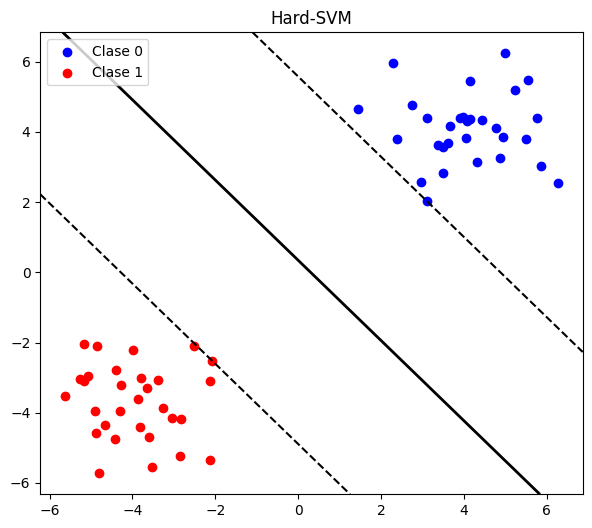
\includegraphics[width=0.35\textwidth]{./figures/hard-svm-1.png}
    \end{center}
\end{frame}

\begin{frame}
\begin{block}{Teorema}
Sea $w$ el vector del hiperplano separador óptimo del problema homogéneo ($b=0$). Sea $I = \{i \in \{1, \dots, m\} : (x_i,y_i) \text{ es vector soporte}\}$, entonces existen $\alpha_1, \dots, \alpha_m$ tales que $w = \sum_{i \in I} \alpha_ix_i$
\end{block}
\vspace{0.5cm}

\underline{Observación:} El problema no homogéneo dado por $D=\{(x_i,y_i)\}$, $x_i \in \mathbb{R}^d$, $y_i \in \{-1, +1\}$ con hiperplano separador $(w, b)$, se puede puede convertir en un problema homogéneo tomando
\[\hat{x}_i = (x_i, 1) \in \mathbb{R}^{d+1} \ \ \ \ \ \ \hat{y_i} = y_i\]
\[\hat{w} = (w,b) \ \ \ \ \ \ \hat{b} =0\]
\end{frame}

\begin{frame}
El hiperplano de margen máximo está determinado exclusivamente por los vectores soporte. Esto hace que el modelo \textit{hard-SVM} sea inestable ya que un pequeño cambio en el conjunto de entrenamiento, como un nuevo dato cerca de la frontera, puede modificar drásticamente el hiperplano solución.\\
\vspace{0.5 cm}
\begin{columns}
    \column{0.5\textwidth}
    \centering
    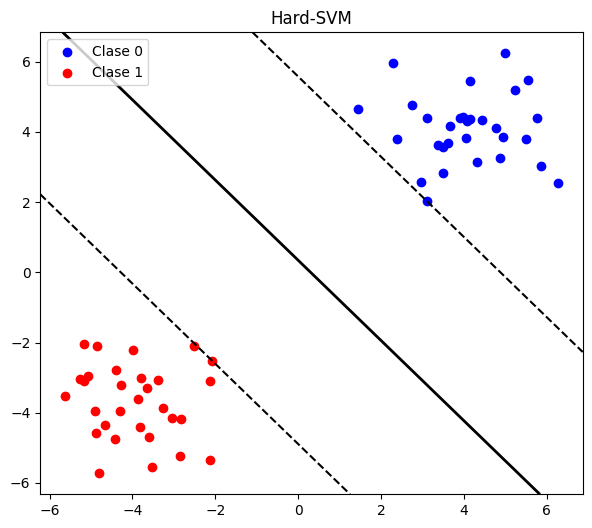
\includegraphics[width=\linewidth]{./figures/hard-svm-1.png}
    
    \column{0.5\textwidth}
    \centering
    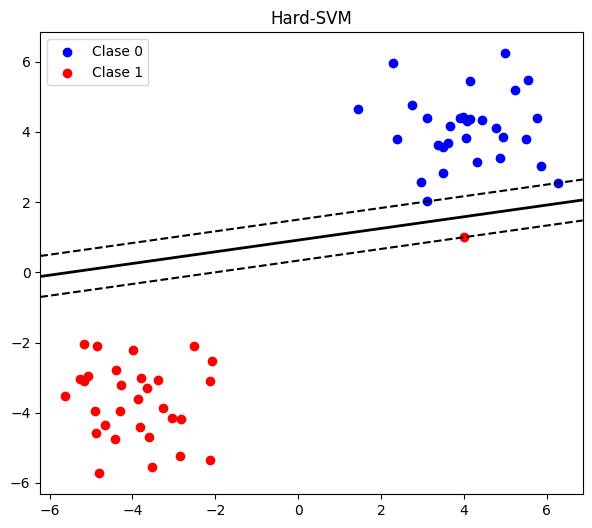
\includegraphics[width=\linewidth]{./figures/hard-svm-2.png}
\end{columns}
\end{frame}

\begin{frame}{Soft-SVM}
Consiste en relajar las condiciones para permitir que se cometan errores al clasificar los datos de entrenamiento. Esto nos permitirá

\begin{enumerate}
    \item Clasificar conjuntos en los que las clases no sean separables por un hiperplano
    \item Evitar el sobreajuste 
\end{enumerate}
\vspace{0.5cm}
Introducimos las variables de holgura $\xi_1, \dots, \xi_m$, $\xi_i \geq 0$
\vspace{0.5cm}
\begin{block}{Algoritmo Soft-SVM}
input: $(x_1,y_1), \dots, (x_m,y_m)$\\ \vspace{0.15cm}
parameter: $\lambda >0$\\ \vspace{0.15cm}
solve: $\min_{w, b, \zeta}(\lambda \|w\|^2 +\frac{1}{m}\sum_{i=1}^m \xi_i)$ \\ \vspace{0.15cm} sujeto a $y_i(\langle w,x_i\rangle+b)\geq 1-\xi_i$, $\xi_i \geq 0$ $\forall i$\\ \vspace{0.15cm}
output: $w$, $b$
\end{block}

\end{frame}

\begin{frame}
\textbf{Interpretación de las variables de holgura:}
\begin{itemize}
    \item $\xi_i = 0$: el punto está bien clasificado y fuera del margen.
    \item $0 < \xi_i < 1$: el punto está dentro del margen, pero bien clasificado.
    \item $\xi_i > 1$: el punto está mal clasificado.
\end{itemize}

\vspace{0.3cm}

\vspace{0.3cm}

\textbf{Interpretación del parámetro $\lambda$}
Controla el equilibrio entre maximizar el margen y permitir errores:
\begin{itemize}
    \item $\lambda$ pequeño: penaliza mucho los errores
    \item $\lambda$ grande : permite más errores
\end{itemize}

\end{frame}




\begin{frame}
\begin{columns}
    \column{0.4\textwidth}
    \centering
    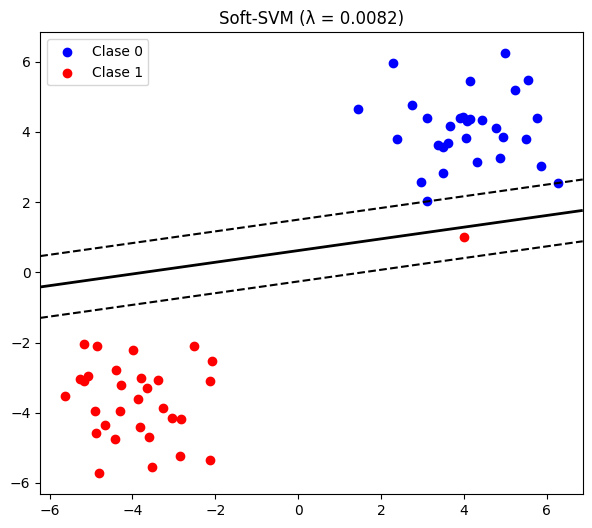
\includegraphics[width=\linewidth]{./figures/soft-svm-1.png}
    
    \column{0.4\textwidth}
    \centering
    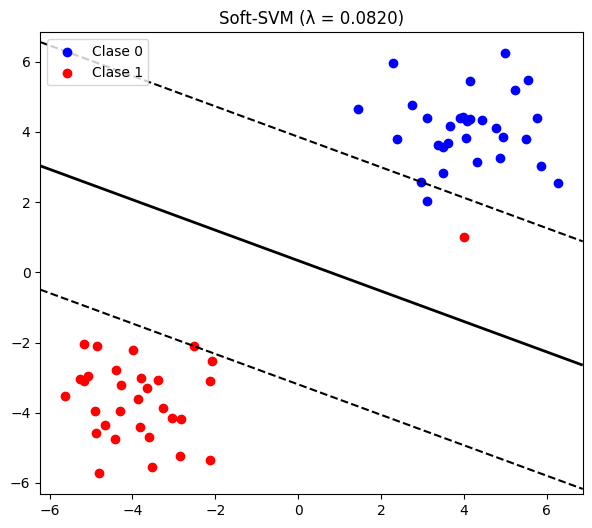
\includegraphics[width=\linewidth]{./figures/soft-svm-2.png}
\end{columns}
\vspace{0.25cm}
\begin{columns}
    \column{0.4\textwidth}
    \centering
    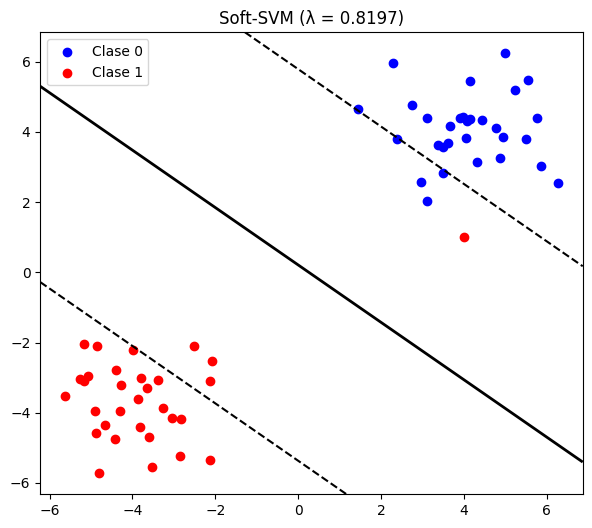
\includegraphics[width=\linewidth]{./figures/soft-svm-3.png}
    
    \column{0.4\textwidth}
    \centering
    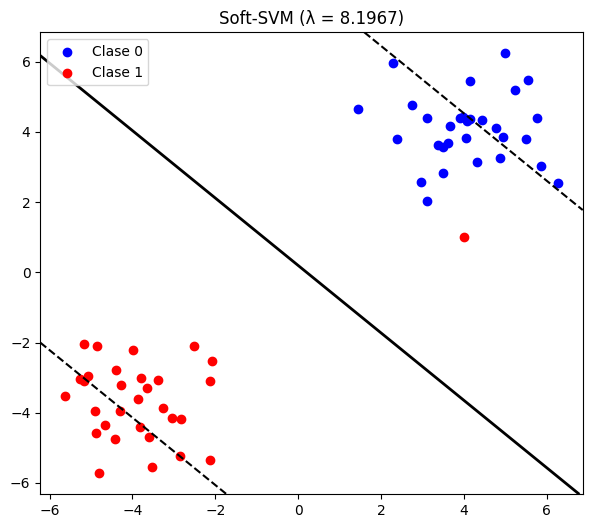
\includegraphics[width=\linewidth]{./figures/soft-svm-4.png}
\end{columns}
\end{frame}

\begin{frame}{Función de error}
\begin{center}$\mathcal{E}_{\mathcal{D}}^{\text{hinge}}(w,b) := \frac{1}{m} \sum_{i=1}^{m} \max \{0, 1 - y_i (\langle w, x_i \rangle + b)\}$
\end{center}
\vspace{0.15cm}
Se tiene que
{\footnotesize
 $$\xi_i := 
\begin{cases}
0 & \text{si } y_i (\langle w, x_i \rangle + b) > 1 \\
1 - y_i (\langle w, x_i \rangle + b) & \text{si no}
\end{cases}$$}\\
\vspace{0.15cm}
El algoritmo soft-SVM es equivalente a optimizar
\begin{center}
    $\underset{(w,b)}{\text{arg mín}} \quad \mathcal{E}_{\text{hinge}}(w,b) + \lambda \|w\|^2$
\end{center}

\vspace{0.15cm}
\underline{Observación:}\\ 
El error empírico $ \mathcal{E}_{\mathcal{D}}(w,b) =  \frac{4}{m}\left|\{i : y_i(\langle w,x_i\rangle + b) < 0\}\right|$ no es convexo $\implies$ puede tener varios mínimos.\\
\vspace{0.25cm}
$\mathcal{E}_{\mathcal{D}}^{\text{hinge}}(w,b) + \lambda\|w\|^2$ es convexa $\forall \mathcal{D}$

\end{frame}



\section{Métodos kernel}

\begin{frame}{Métodos kernel}
    Si nuestra muestra \(\mathcal{D} = \{(y_i,x_i)\}_{i=1}^m\) no es separable y \textit{soft-SVM} no proporciona un resultado satifactorio, podemos incrustar nuestra muestra, mediante una aplicación \(\phi\), en un espacio de dimensión mayor en el que \(\{(y_i,\phi(x_i))\}_{i=1}^m\) sí sea separable.

    \vspace{0.2in}

\centering
\resizebox{\textwidth}{!}{%
\begin{tikzpicture}[
    >=Latex,
    line cap=round,
    line join=round,
    font=\small,
    axis/.style={->,thick},
    classA/.style={circle,fill=blue!70!black,draw=white,inner sep=1.9pt},
    classB/.style={circle,fill=orange!90!red,draw=white,inner sep=1.9pt},
    lab/.style={font=\footnotesize}
]

%============================================================
% PANEL IZQUIERDO: R^2
%============================================================
\coordinate (O2) at (0,0);

% ejes sin etiquetas
\draw[axis] ($(O2)+(-1.8,0)$) -- ($(O2)+(1.9,0)$);
\draw[axis] ($(O2)+(0,-1.7)$) -- ($(O2)+(0,1.9)$);

% clase interior
\foreach \xx/\yy in {
  0.00/0.00,
  0.16/0.10,
  -0.18/0.14,
  0.12/-0.20,
  -0.22/-0.08,
  0.26/-0.03,
  -0.06/0.24,
  0.31/0.12,
  -0.30/0.06,
  0.05/-0.31,
  -0.12/-0.26,
  0.22/0.27
}{
  \node[classA] at ($(O2)+(\xx,\yy)$) {};
}

% clase exterior (corona)
\foreach \xx/\yy in {
  1.10/0.00,
  0.92/0.52,
  0.55/0.96,
  0.00/1.13,
  -0.58/0.95,
  -0.95/0.50,
  -1.12/0.00,
  -0.95/-0.50,
  -0.58/-0.97,
  0.00/-1.14,
  0.60/-0.94,
  0.96/-0.56,
  0.78/0.83,
  -0.78/0.82
}{
  \node[classB] at ($(O2)+(\xx,\yy)$) {};
}

\node[lab] at ($(O2)+(0,-2.0)$) {$\mathbb{R}^2$};

%============================================================
% FLECHA CENTRAL
%============================================================
\draw[->, very thick]
  (2.5,0.0) -- (6.0,0.0)
  node[midway, above=4pt] {$\phi(x)=\left(x,\frac{1}{1+\|x\|^2}\right)$};

%============================================================
% PANEL DERECHO: R^3
%============================================================
\begin{scope}[shift={(8.55,-0.82)}, x={(1.65cm,0cm)}, y={(-1.20cm,0.40cm)}, z={(0cm,2.35cm)}]

% ejes sin etiquetas
\draw[axis] (0,0,0) -- (2.00,0,0);
\draw[axis] (0,0,0) -- (0,1.45,0);
\draw[axis] (0,0,0) -- (0,0,1.10);

% dibujamos primero la clase exterior
\foreach \xx/\yy in {
  1.10/0.00,
  0.92/0.52,
  0.55/0.96,
  0.00/1.13,
  -0.58/0.95,
  -0.95/0.50,
  -1.12/0.00,
  -0.95/-0.50,
  -0.58/-0.97,
  0.00/-1.14,
  0.60/-0.94,
  0.96/-0.56,
  0.78/0.83,
  -0.78/0.82
}{
  \pgfmathsetmacro{\rrsq}{\xx*\xx+\yy*\yy}
  \pgfmathsetmacro{\zz}{1/(1+\rrsq)}
  \node[classB] at (\xx,\yy,\zz) {};
}

% luego la clase interior
\foreach \xx/\yy in {
  0.00/0.00,
  0.16/0.10,
  -0.18/0.14,
  0.12/-0.20,
  -0.22/-0.08,
  0.26/-0.03,
  -0.06/0.24,
  0.31/0.12,
  -0.30/0.06,
  0.05/-0.31,
  -0.12/-0.26,
  0.22/0.27
}{
  \pgfmathsetmacro{\rrsq}{\xx*\xx+\yy*\yy}
  \pgfmathsetmacro{\zz}{1/(1+\rrsq)}
  \node[classA] at (\xx,\yy,\zz) {};
}

\node[lab] at (0.15,-1.55,0) {$\mathbb{R}^3$};

\end{scope}
\end{tikzpicture}%
}
    
\end{frame}

\begin{frame}
    El problema es que no tenemos por qué saber la estructura de los datos y, por tanto, qué \(\phi\) escoger. Para lidiar con esto, usamos la teoría de espacios de Hilbert de núcleo reproductor (RKHS).

    \vspace{0.2in}
    
    \begin{itemize}
        \item Queremos encontrar \(f:X\subset\mathbb{R}^d\to\mathbb{R}^N\) continua.
        \item Nuestra \(\phi\) será su grafo: \(\phi(x) := (x,f(x))\).
        \item Entonces \(K^f(x,y) := \langle x,y \rangle_{\mathbb{R}^d} + \langle f(x),f(y) \rangle_{\mathbb{R}^N}\) es un núcleo de Mercer.
        \item Además, \(K^f(x,y) = \langle \phi(x),\phi(y)\rangle_{\mathbb{R}^d\times\mathbb{R}^N}\).
    \end{itemize}

    \vspace{0.2in}
    
    El siguiente teorema, aunque parezca técnico, nos va a servir para quitarnos la dependencia de \(\phi\) en nuestro algoritmo.
    
\end{frame}

\begin{frame}
    \begin{block}{Teorema}
        Sea 
        \[
        \mathcal{H}_\phi := \{\xi:X\to\mathbb{K} \mid \exists w \in \operatorname{span}\{\phi(x)\} : \xi(x) = \xi_w(x) := \langle w,\phi(x) \rangle_{\mathbb{R}^d\times\mathbb{R}^N}\} 
        \] 
        dotado del producto escalar:
        \(
        \langle \xi_{w_1},\xi_{w_2} \rangle_{\mathcal{H}_\phi} := \langle w_1,w_2 \rangle_{\mathbb{R}^d\times\mathbb{R}^N}.
        \)
        Entonces,
        \[
        \mathcal{H}_\phi \equiv \mathcal{H}_{K^f}
        \]
    \end{block}

    \begin{proof}
        Por construcción, la aplicación
    \[
    \begin{aligned}
        L : \operatorname{span}\{\phi(x)\} &\longrightarrow \mathcal{H_\phi} \\
        w &\longmapsto \langle w,\phi(\cdot) \rangle_{\mathbb{R}^d\times\mathbb{R}^N}
    \end{aligned}
    \]
    es una isometría lineal biyectiva. Por tanto,
    \[
    \xi(x) = \langle w,\phi(x) \rangle_{\mathbb{R}^d\times\mathbb{R}^N} = \langle L^{-1}\xi,\phi(x) \rangle_{\mathbb{R}^d\times\mathbb{R}^N} = \langle \xi,L\phi(x) \rangle_{\mathcal{H}_\phi} = \langle \xi,K_x^f \rangle_{\mathcal{H}_\phi},
    \]
    que es la propiedad de reproducción. Por unicidad de \(\mathcal{H}_{K^f}\), hemos terminado.
    \end{proof}
    
\end{frame}

\begin{frame}
    La aplicación directa de este teorema es que optimizar la aplicación
    \[
    \mathscr{L}_{\mathcal{D}}^\phi(w) = \frac{1}{m} \sum_{i=1}^m \max\{0,1-y_i \langle w,\phi(x_i) \rangle_{\mathbb{R}^d\times\mathbb{R}^N}\} + \lambda \lVert w \rVert_{\mathbb{R}^d\times\mathbb{R}^N}^2
    \]
    sea equivalente a optimizar
    \begin{equation} \label{opK}
        \mathscr{L}_{\mathcal{D}}^K(\xi) = \frac{1}{m} \sum_{i=1}^m \max\{0,1-y_i \xi(x_i)\} + \lambda \lVert \xi \rVert_{\mathcal{H}_K}^2.
    \end{equation}

    El funcional \eqref{opK} no depende de \(\phi\), sólo del RKHS elegido. Por tanto, si existen unos espacios \(\mathcal{H}_K\) ``universales'', podremos usarlos para separar de forma satisfactoria nuestra muestra sin tener que escoger de forma arbitraria una aplicación \(\phi\). Sin embargo, esto introduce un nuevo problema, tenemos que optimizar en un espacio que puede ser de dimensión infinita. Para solventar este inconveniente, usamos el Teorema del representador.
    
\end{frame}

\begin{frame}

\begin{block} {Teorema del representador}
    Sea \(K\) un núcleo de Mercer sobre \(X \times X\), \(\mathcal{H}_K\) su RKHS asociado y \(x_1, \dots, x_m \in X\). Consideramos el problema
    
    \begin{equation}\label{RT}
        \min_{\xi\in\mathcal{H}_K} \frac{1}{m} \sum_{i=1}^m \max\{0,1-y_i\xi(x_i)\} + \lambda \lVert \xi \rVert_{\mathcal{H}_K}^2.
    \end{equation}
    
    Entonces \(\exists \alpha_1, \dots, \alpha_m \in \mathbb{K}\) tales que
    \[
    \xi^\ast(x) = \sum_{i=1}^m \alpha_i K(x_i,x)
    \]
    cumple \eqref{RT}.
\end{block}

\vspace{0.1in}

Es decir, realmente no estamos optimizando sobre un espacio de dimensión infinita porque se puede encontrar un mínimo en \(\operatorname{span}\{K_{x_1}, \dots, K_{x_m}\}\).
    
\end{frame}

\begin{frame}
    \begin{proof}
        Sea \(V = \operatorname{span}\{K_{x_1}, \dots, K_{x_m}\}\). Como \(V\) es de dimensión finita, es cerrado y, por tanto, podemos aplicar el teorema de la descomposición ortogonal:
        \[
        \forall \xi \in \mathcal{H}_K \hspace{0.1in} \xi = \xi_V + \xi_{V^\perp}
        \]
        Por la propiedad de reproducción,
        \[
        \xi(x_i) = \langle \xi,K_{x_i} \rangle_{\mathcal{H}_K} = \langle \xi_V,K_{x_i} \rangle_{\mathcal{H}_K} = \xi_V(x_i).
        \]
        Además,
        \[
        \lVert \xi \rVert_{\mathcal{H}_K}^2 = \lVert \xi_V \rVert_{\mathcal{H}_K}^2 + \lVert \xi_{V^\perp} \rVert_{\mathcal{H}_K}^2 \geq \lVert \xi_V \rVert_{\mathcal{H}_K}^2 
        \]
        Entonces,
        \[
        \mathscr{L}_{\mathcal{D}}^K(\xi_V) \leq \mathscr{L}_{\mathcal{D}}^K(\xi).
        \]
    \end{proof}
\end{frame}

\begin{frame}
    Este teorema nos brinda la reformulación definitiva de nuestro problema. Si \(\xi \in V_{\mathcal{D}}\), entonces
    \[
    \xi(x_i) = \sum_{j=1}^m \alpha_j K(x_i,x_j), \hspace{0.3in}
    \lVert \xi \rVert_{\mathcal{H}_K}^2 = \sum_{i,j=1}^m \alpha_i \overline{\alpha}_j K(x_i,x_j).
    \]
    Si definimos \((M_K^{\mathcal{D}})_{i,j} = K(x_i,x_j)\), entonces podemos escribir el funcional a minimizar como:
    \[
        \mathscr{L}_{\mathcal{D}}^K(\alpha) = \frac{1}{m} \sum_{i=1}^m \max\{0,1-y_i (M_K^{\mathcal{D}}\alpha)_i\} + \lambda \langle \alpha, M_K^{\mathcal{D}} \alpha\rangle_{\mathbb{K}^m}.
    \]
    Por último, si \(\alpha^\ast = \underset{\alpha \in \mathbb{K}^m} {\mathrm{arg\,\min}} \hspace{0.05in} \mathscr{L}_{\mathcal{D}}^K(\alpha)\), el clasificador es
    \[
    f(x) = \operatorname{signo} \left( \sum_{j=1}^m \alpha_j^\ast K(x_j,x) \right).
    \]
\end{frame}

\begin{frame}
    Para terminar, retomamos la discusión sobre los RKHS universales.
    \begin{block}{Propiedad universal}
       Decimos que un RKHS es universal si \(\forall A, B \subset X\) compactos y disjuntos \(\exists f \in\) RKHS tal que \(f(A) > 0\), \(f(B) < 0\).
    \end{block}
    Básicamente estamos imponiendo que nuestro espacio sea capaz de separar cualquier muestra. Debido a esto, casi siempre vamos a querer usar núcleos universales en la práctica. Para encontrarlos usamos la siguiente proposición.
    \begin{block}{Proposición}
        Sea \(X\) un espacio métrico compacto y sea \(V \subset C(X)\) un conjunto denso en norma infinito. Entonces \(V\) cumple la propiedad universal.
    \end{block}
    De esta forma se puede demostrar que la función gaussiana de base radial
    \[
    K(x,y) = e^{-\gamma\lVert x-y \rVert^2}
    \]
    es un kernel universal si \(\gamma > 0\).
\end{frame}

\section{Costes asimétricos}

\begin{frame}{Costes Asimétricos: cribado de cáncer de mama}
  En cribado de cáncer de mama los errores tienen consecuencias diferentes.

  \vspace{0.12in}

  Fijamos etiquetas $y \in \{-1,+1\}$:
  \[
  y=+1 \;\text{(maligno)}, \qquad y=-1 \;\text{(benigno)}.
  \]

  \vspace{0.05in}

  \begin{itemize}
    \item FP: $y=-1$ y $\hat y=+1$ (alarma innecesaria).
    \item FN: $y=+1$ y $\hat y=-1$ (caso clínicamente más grave).
  \end{itemize}

  Frente al objetivo estándar (minimizar error 0-1), usamos pérdida coste-sensible:
  \[
  \ell_c(y,\hat y)=
  \begin{cases}
    0, & y=\hat y,\\
    c_{FP}, & y=-1,\,\hat y=+1,\\
    c_{FN}, & y=+1,\,\hat y=-1.
  \end{cases}
  \]

  Riesgo esperado y coste medio empírico:
  \[
  \mathcal{R}_c(f)=\mathbb{E}[\ell_c(Y,f(X))], \qquad
  \widehat{\mathcal{R}}_c(f)=\frac{1}{m}\big(c_{FP}\,FP(f)+c_{FN}\,FN(f)\big).
  \]
  En este contexto suele imponerse $c_{FN}>c_{FP}$.
\end{frame}

\begin{frame}{Soft-SVM: efecto de $C$}
  Modelo primal de \textit{soft-SVM}:
  \[
  \min_{w,b,\xi}\;\frac{1}{2}\norm{w}^2 + C\sum_{i=1}^m \xi_i
  \quad \text{s.a.} \quad
  y_i(\langle w,x_i\rangle+b)\ge 1-\xi_i,\; \xi_i\ge 0.
  \]

  \textbf{Notación:} salvo constantes de normalización, en \texttt{sklearn} se usa
  $C\propto\frac{1}{\lambda}$.
  
  \vspace{0.02in}
  \textbf{Margen geométrico:} la distancia de un vector soporte a la frontera es
  $\frac{1}{\norm{w}}$.

  \vspace{0.05in}
  \begin{itemize}
    \item $C\uparrow$: se penalizan más las violaciones ($\xi_i$), suele crecer $\norm{w}$ y el margen tiende a estrecharse.
    \item $C\downarrow$: pesa más la regularización, suele bajar $\norm{w}$ y el margen tiende a ampliarse.
    \item Al variar $C$, cambian la solución $w^*$ y el conjunto de vectores soporte activos.
  \end{itemize}

  
\end{frame}

\begin{frame}{Soft-SVM con costes asimétricos: $C_+$ y $C_-$}
  Modelo primal con costes asimétricos:
  \[
  \min_{w,b,\xi}\;\frac{1}{2}\norm{w}^2
  + C_+\sum_{i:y_i=+1}\xi_i
  + C_-\sum_{i:y_i=-1}\xi_i
  \]
  con las mismas restricciones de margen.

  \vspace{0.05in}

  \begin{itemize}
    \item Si $C_+>C_-$, se penalizan más violaciones en la clase $y=+1$.
    \item Efecto de $C_\pm$: subir $C_+$ (o bajar $C_-$) desplaza la frontera para proteger más a los positivos.
    \item Efecto típico: disminuyen FN y aumentan FP; lo contrario si se prioriza la clase negativa.
  \end{itemize}

\end{frame}

\begin{frame}{Comparativa visual: $C_+=0.5$ vs $C_+=10$}
  \begin{figure}
    \centering
    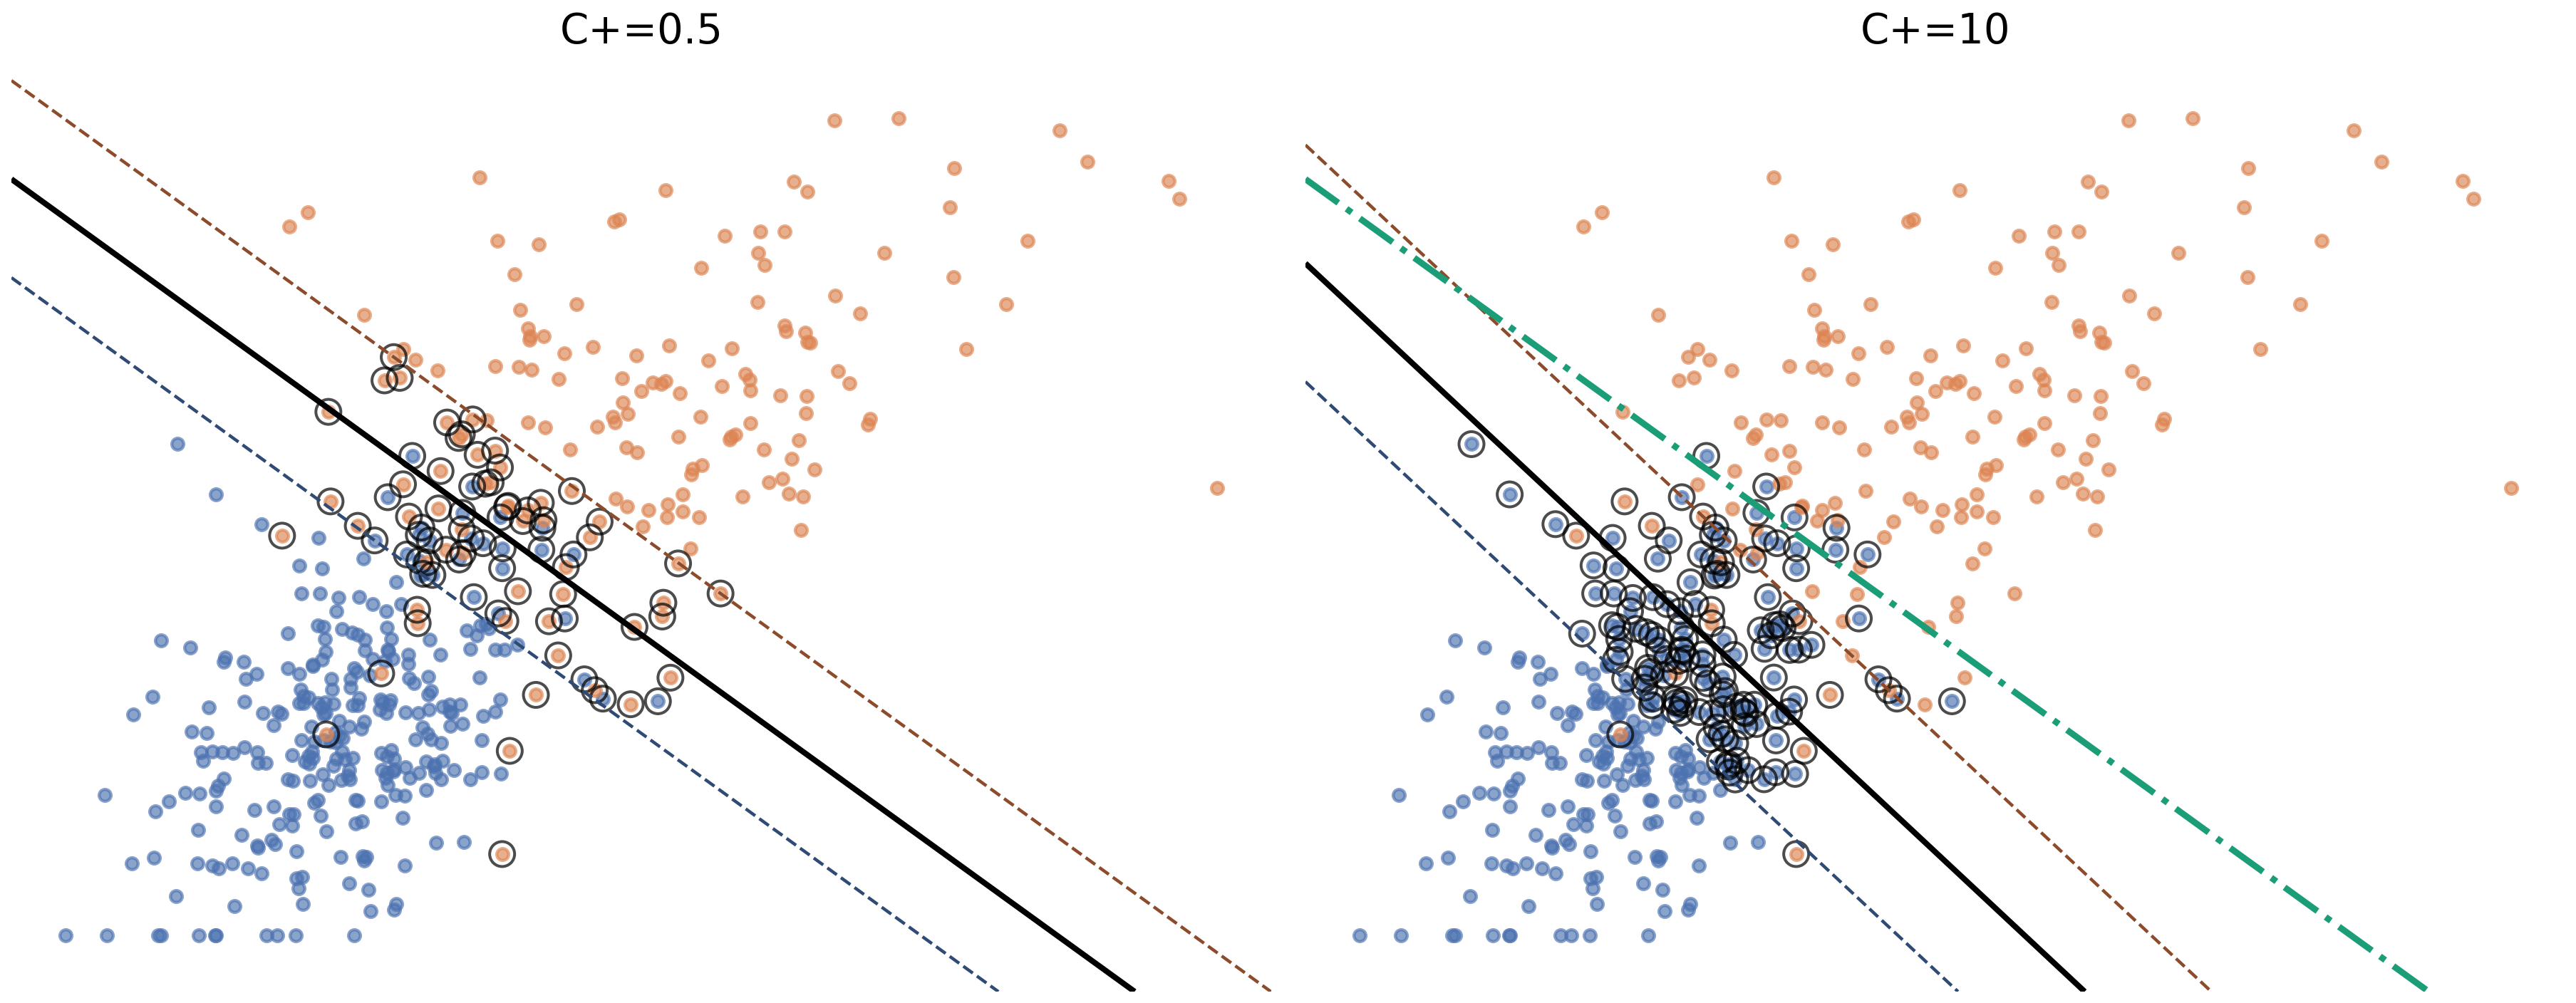
\includegraphics[width=0.98\textwidth]{./figures/comparativa_cplus_minimalista_sin_fondo.png}
  \end{figure}
\end{frame}



\section{Clasificación lineal multiclase}

\begin{frame}{Clasificación lineal multiclase}
    Podemos extender el algoritmo SVM para clasificar en $k \in \mathbb{N}$ clases. Para $Y = \{1, \dots, k\}$ y $\mathcal{D} = \{(x_i,y_i)\}_{i=1}^m \subset X \times Y$, definimos:

    \begin{itemize}
        \item \textbf{Clasificación:} $f \colon X \to Y$.
        \item \textbf{Error de clasificación:} $\ds \mathcal{E}[f] = \int_X \mathbb{P}(Y \neq f(x) \mid x) \odif{\rho_X(x)}$.
        \item \textbf{Error empírico:} $\ds \mathcal{E}_{\mathcal{D}} [f] = \frac{1}{m} \abs{\{i \in \{1, \dots, m\} : f(x_i) \neq y_i\}}$.
    \end{itemize}

    \vspace{0.5cm}
    
    Tres enfoques para la clasificación multiclase:
    \begin{enumerate}
        \item \textbf{One-vs-Rest} (también conocido como One-vs-All).
        \item \textbf{One-vs-One.}
        \item \textbf{SVM de Crammer–Singer.}
    \end{enumerate}
\end{frame}

\subsection{Reducción al caso binario}

\begin{frame}{Reducción al caso binario: One-vs-Rest}
    Para cada clase $j \in Y$, entrenamos un clasificador binario que distingue la clase $j$ del resto.
    \begin{enumerate}
        \item $\mathcal{D}_j = \left\{(x_i, \sigma_j(y_i))\right\}_{i=1}^m$, donde $\sigma_j(y) = \begin{cases}
          +1 & \text{si } y = j, \\
          -1 & \text{si } y \neq j.
        \end{cases}$
        \item Entrenamos un SVM binario en $\mathcal{D}_j$ para obtener $(w_j^*, b_j^*) \in \mathbb{R}^d \times \mathbb{R}$ que definen $\xi_j(x) = \langle w_j^*, x \rangle + b_j^*$.
    
        \vspace{0.5cm}
    
        Las $\xi_j$ se denominan \textbf{funciones de puntuación} o \textit{scores} porque miden la confianza del clasificador en asignar a $x$ la clase $j$.
      \end{enumerate}
      \vspace{0.5cm}
      La clasificación final es $\ds f(x) = \arg\max_{j \in Y} \xi_j(x)$.
\end{frame}

\begin{frame}
    \begin{figure}[h!]
      \centering
      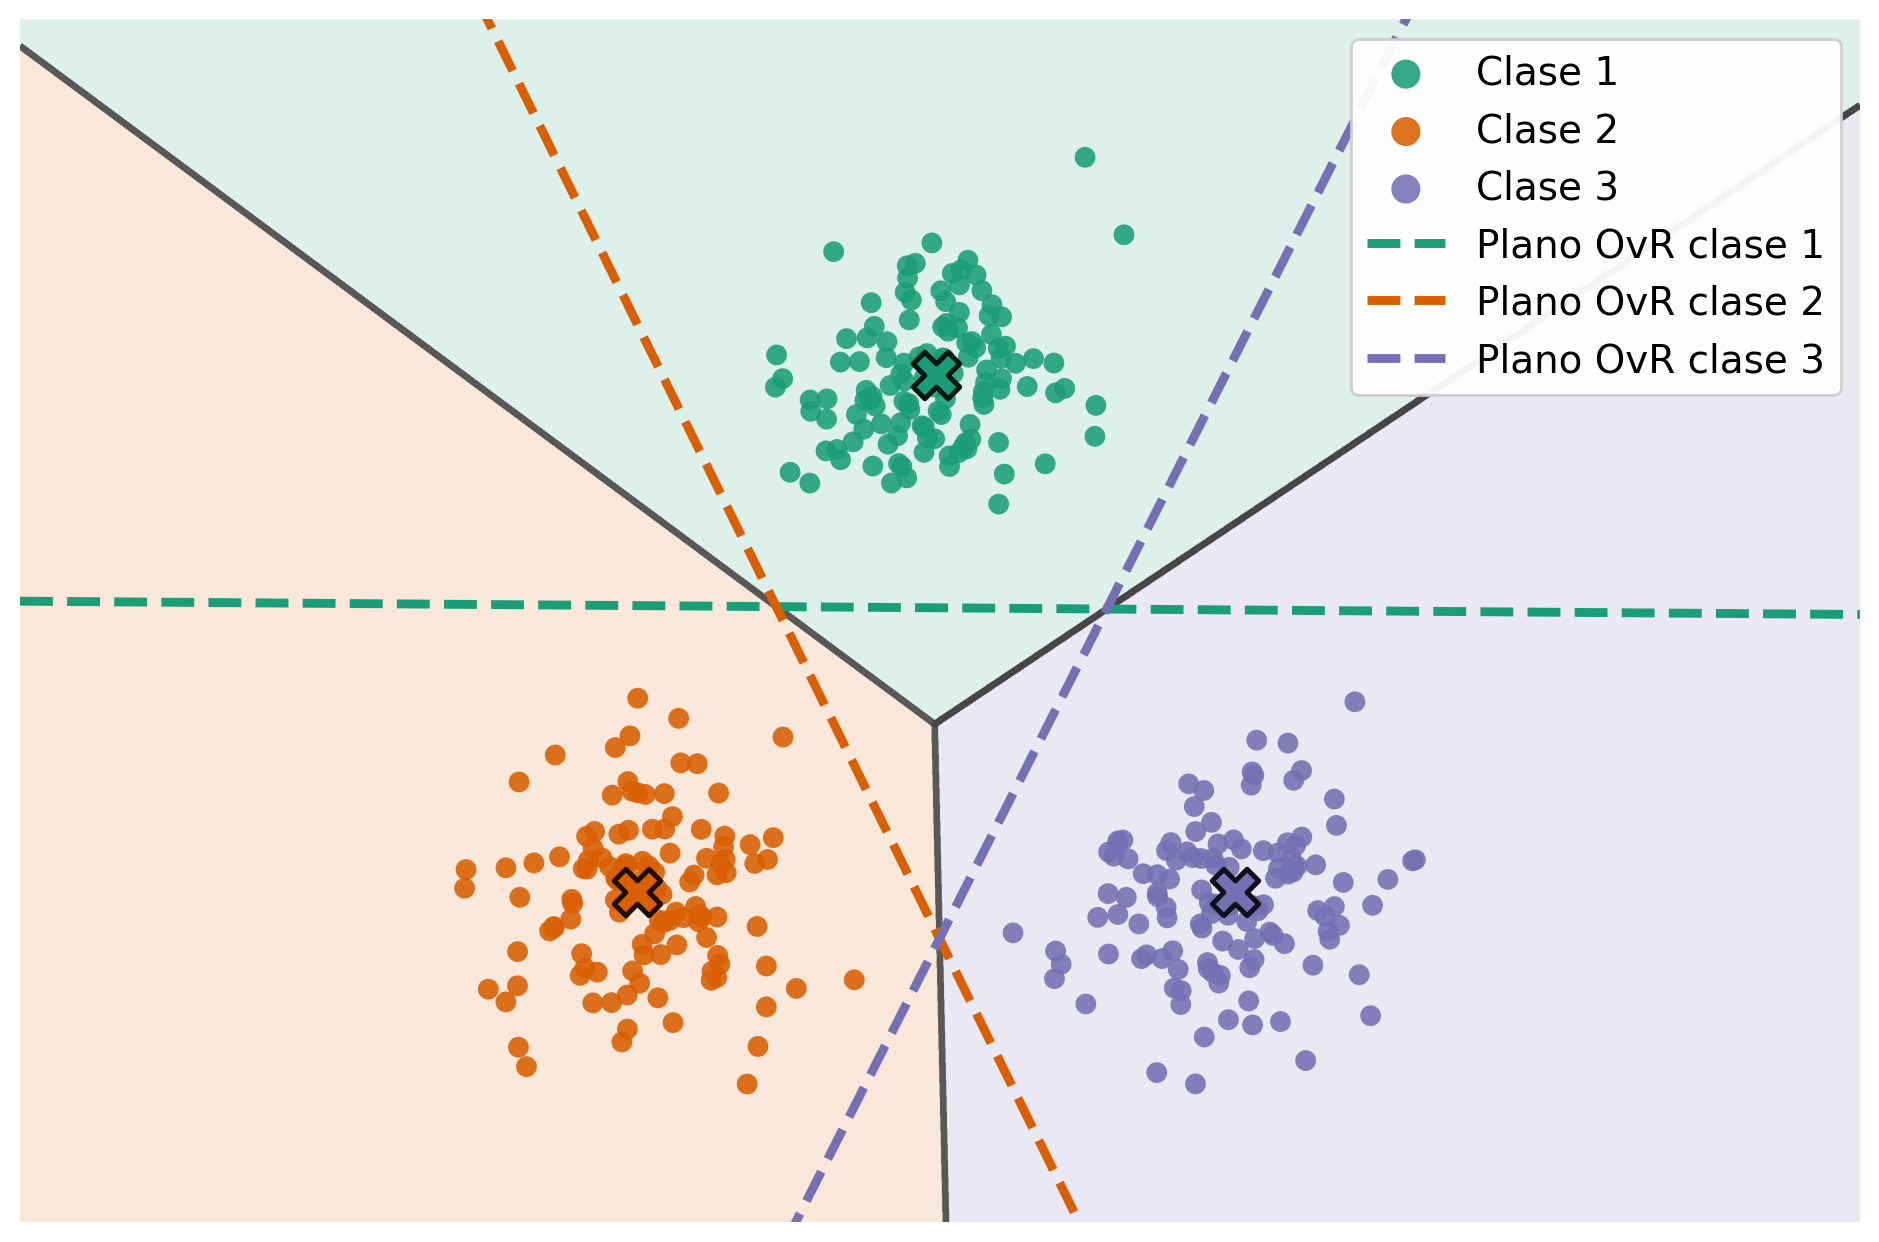
\includegraphics[width=0.85\textwidth]{./figures/ovr_tres_nubes.png}
      \caption{Ejemplo sintético en $\mathbb{R}^2$ y regiones de decisión de una SVM lineal OvR.}
      \label{fig:ovr-tres-nubes}
    \end{figure}
\end{frame}

\begin{frame}{Reducción al caso binario: One-vs-One}
    Para cada par de clases $j, \ell \in Y$ (con $j < \ell$), entrenamos un clasificador binario que distingue entre ellas.
    \vspace{0.5cm}
    \begin{enumerate}
        \item $\mathcal{D}_{j\ell} = \left\{(x_i, \sigma_{j\ell}(y_i)): i \in I_{j} \cup I_{\ell}\right\}$, donde $I_j = \{i \in \mathbb{N}_m : y_i = j\}$, $I_\ell = \{i \in \mathbb{N}_m : y_i = \ell\}$ y $\sigma_{j\ell}(y) = \begin{cases}
          +1 & \text{si } y = j, \\
          -1 & \text{si } y = \ell.
        \end{cases}$
        \item Entrenamos un SVM binario en $\mathcal{D}_{j\ell}$ para obtener $(w_{j\ell}^*, b_{j\ell}^*) \in \mathbb{R}^d \times \mathbb{R}$ que definen $\xi_{j\ell}(x) = \langle w_{j\ell}^*, x \rangle + b_{j\ell}^*$.
    \end{enumerate}
    \vspace{0.5cm}
    Para clasificar $x$, cada clasificador binario emite un voto a la clase que predice. La clasificación final es la clase con más votos:
    \[
    f(x) = \arg\max_{j \in Y} \left[ \sum_{\ell \in Y \setminus \{j\}} \ind_{\{\xi_{j\ell}(x) > 0\}} \right].
    \]
\end{frame}

\begin{frame}{OvR vs OvO}
  \centering
  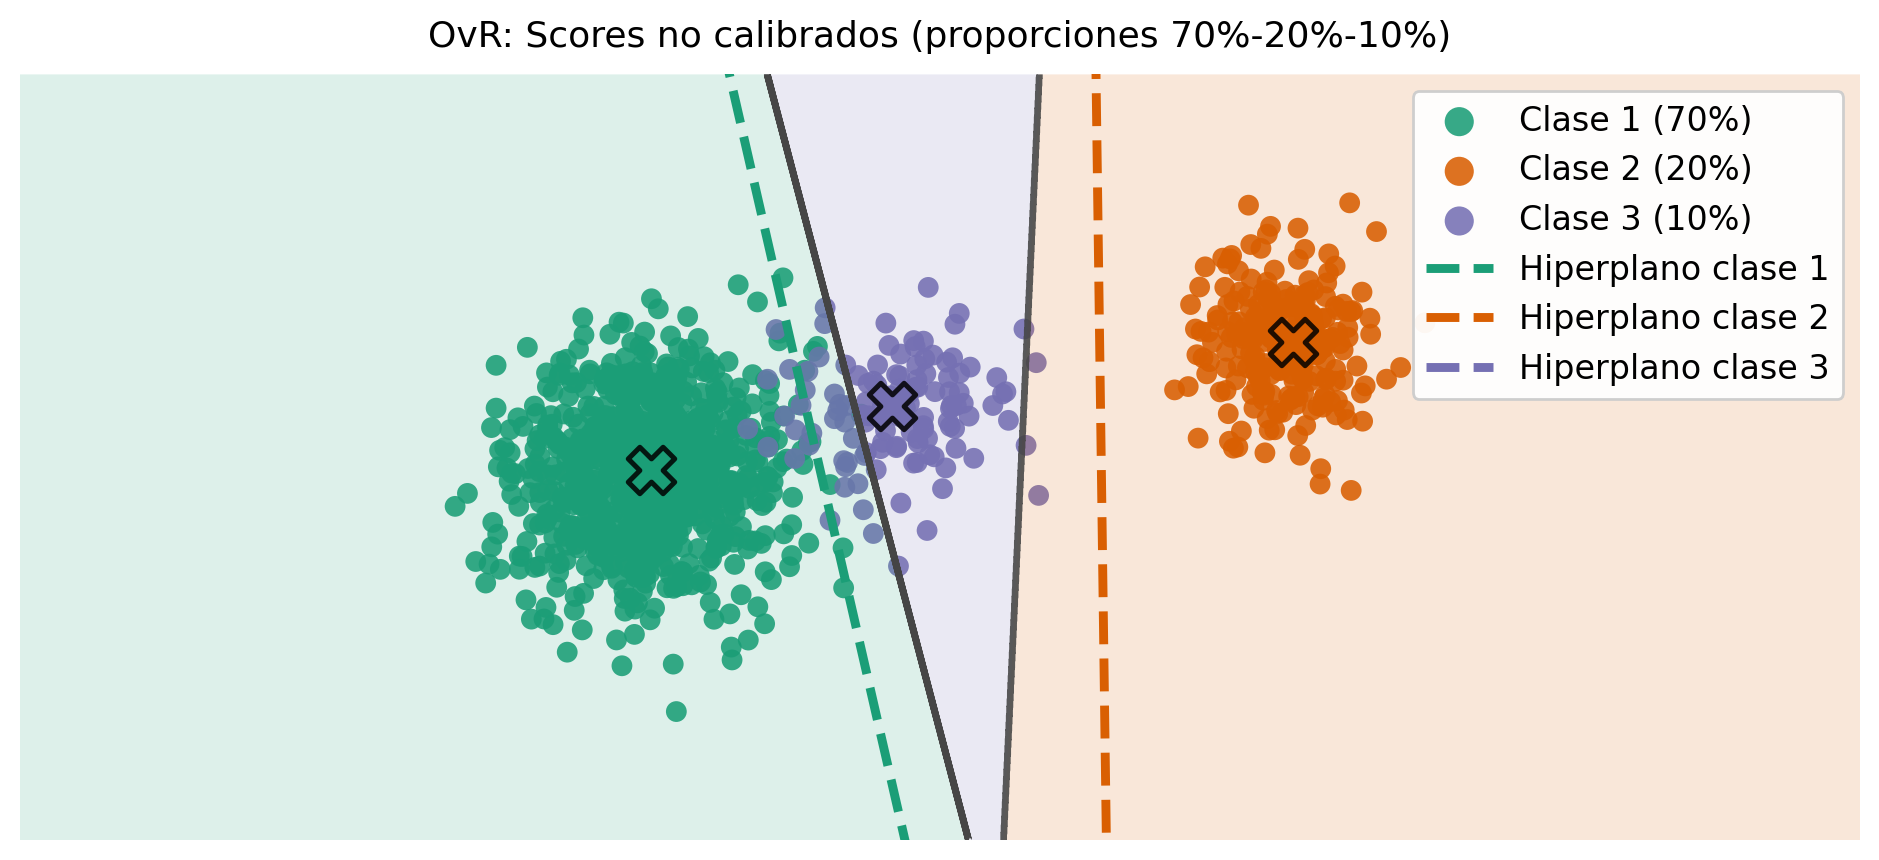
\includegraphics[width=0.72\textwidth]{./figures/ovr_desbalanceado.png}
  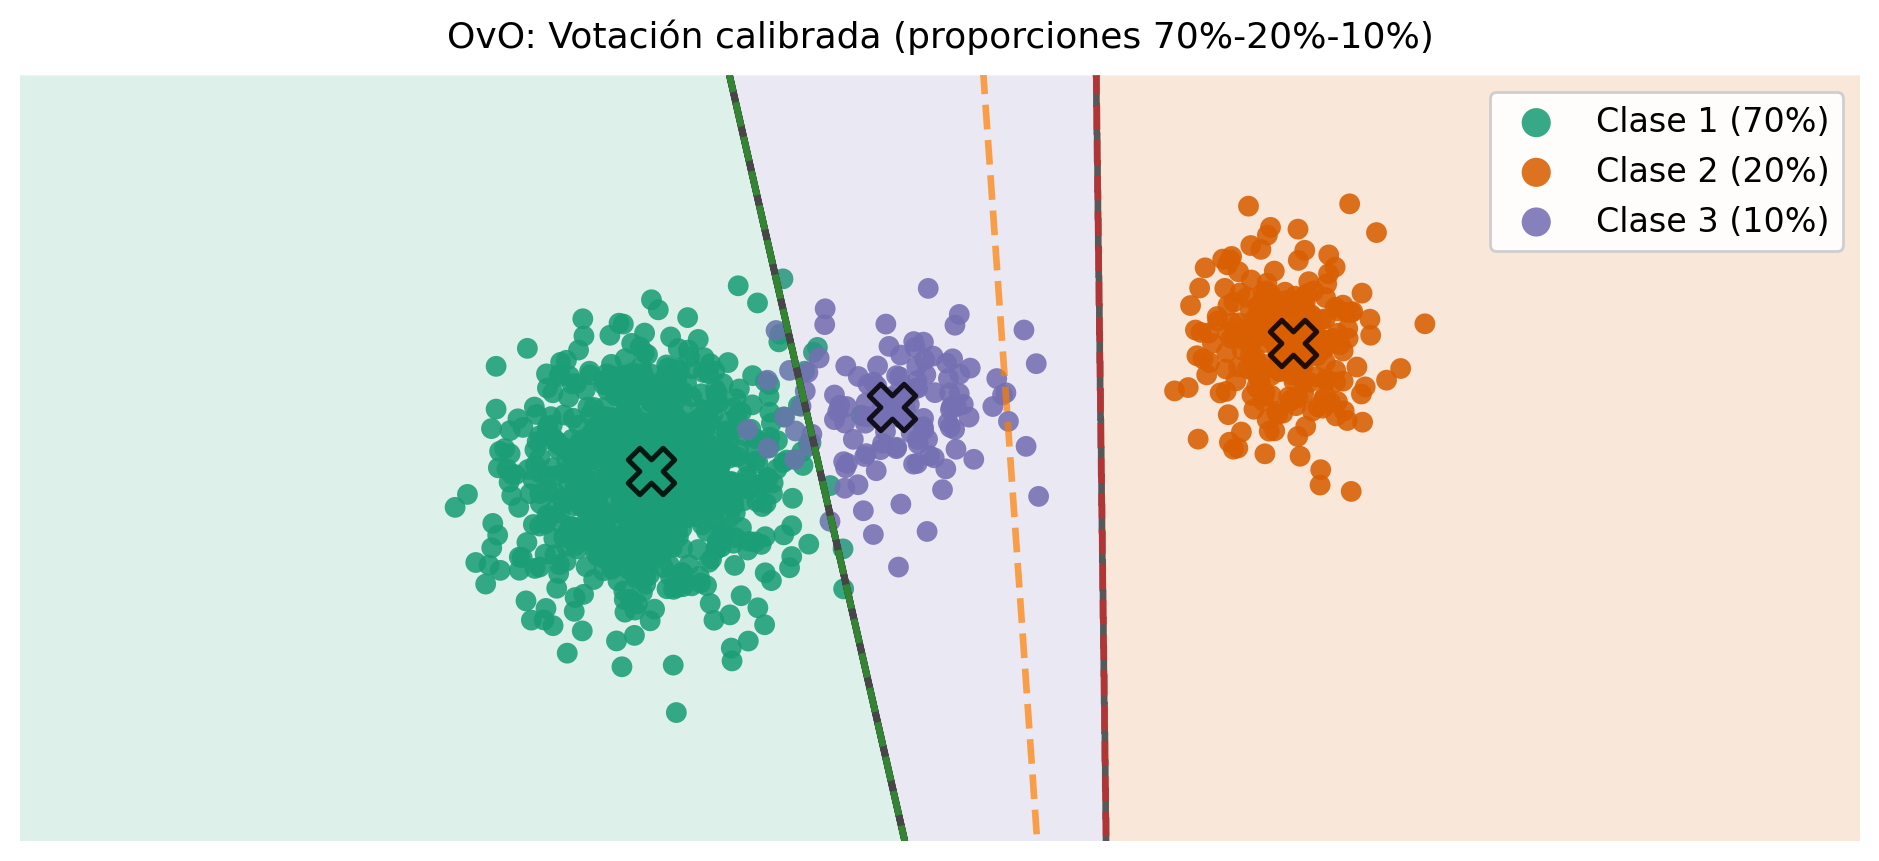
\includegraphics[width=0.72\textwidth]{./figures/ovo_desbalanceado.png}
\end{frame}


\begin{frame}{Formulación directa: SVM de Crammer–Singer}
    En lugar de entrenar múltiples clasificadores binarios, entrenamos un clasificador multiclase directamente.

    \vspace{0.5cm}
    \begin{itemize}
        \item Para cada clase $j \in Y$, queremos una función de puntuación $\xi_j$ dada por $\xi_j(x) = \langle w_j, x \rangle + b_j$ donde $w_j \in \mathbb{R}^d$ y $b_j \in \mathbb{R}$.
        \vspace{0.5cm}

        Entonces, el clasificador vendrá dado por $\ds f(x) = \arg\max_{j \in Y} \xi_j(x)$.
        \item Queremos minimizar la pérdida \textit{hinge} multiclase:
        \[
        \mathcal{E}_\mathcal{D} = \frac{1}{m} \sum_{i=1}^m \max_{j \neq y_i} \max \left\{0, 1 + \xi_j(x_i) - \xi_{y_i}(x_i) \right\}.
        \]
    \end{itemize}
\end{frame}

%\begin{itemize}
  %\item Your introduction goes here!
  %\item Use \texttt{itemize} to organize your main points.
%\end{itemize}

%\vskip 1cm

%\begin{block}{Examples}
%Some examples of commonly used commands and features are included, to help %you get started.
%\end{block}



%\subsection{Tables and Figures}

%\begin{frame}{Tables and Figures}

%\begin{itemize}
%\item Use \texttt{tabular} for basic tables --- see Table~\ref{tab:widgets}, for example.
%\item You can upload a figure (JPEG, PNG or PDF) using the files menu. 
%\item To include it in your document, use the \texttt{includegraphics} %command (see the comment below in the source code).
%\end{itemize}

% Commands to include a figure:
%\begin{figure}
%\includegraphics[width=\textwidth]{your-figure's-file-name}
%\caption{\label{fig:your-figure}Caption goes here.}
%\end{figure}

%\begin{table}
%\centering
%\begin{tabular}{l|r}
%Item & Quantity \\\hline
%Widgets & 42 \\
%Gadgets & 13
%\end{tabular}
%\caption{\label{tab:widgets}An example table.}
%\end{table}

%\end{frame}

%\subsection{Mathematics}

%\begin{frame}{Readable Mathematics}

%Let $X_1, X_2, \ldots, X_n$ be a sequence of independent and identically distributed random variables with $\text{E}[X_i] = \mu$ and $\text{Var}[X_i] = \sigma^2 < \infty$, and let
%\[ S_n = \frac{X_1 + X_2 + \cdots + X_n}{n}
%      = \frac{1}{n}\sum_{i}^{n} X_i \]
%denote their mean. Then as $n$ approaches infinity, the random variables $\sqrt{n}(S_n - \mu)$ converge in distribution to a normal $\mathcal{N}(0, \sigma^2)$.

%\end{frame}

\end{document}